\section{提案手法}
\label{sec:Proposed}
本研究はDPDKのRun-to-Completionモデルを用いたL2分散計算環境を提案する.本章では,その概要としてDPDKによるL2通信を用いることとRun-to-Completionモデルを採用することについて述べる.

\subsection{DPDKによるL2通信の使用}
第\ref{sec:Problem}章で述べたとおり,TCP/IPによる通信ではルーティング,誤り制御,順序制御といった制御が行われる.しかし,第\ref{sec:Background}章で述べた本研究が提案する分散計算環境の前提を踏まえると,これらの制御はオーバーヘッドである.

カーネルによるパケットI/O処理は,一定時間に受信するパケットの量が増えると,コンテキストスイッチが増加して,割り込み以外の処理時間が相対的に少なくなる.また,ユーザ空間のアプリケーションがパケットにアクセスするには,受信したパケットをカーネル空間からユーザ空間にコピーしなければならない.そのため,カーネルのパケットI/O処理はDPDKのパケットI/O処理に比べて低速である.

そこで,本研究では分散計算環境の計算機間の通信にDPDKによるL2通信を用いる.これによって,TCP/IPによるさまざまな通信処理のオーバーヘッドを低減するとともに,カーネルによるパケットI/O処理に比べて高速なパケットI/O処理を用いることができる.

\subsection{Run-to-Completionモデルの採用}
第\ref{sec:DPDK}章で述べたとおり,DPDKのPipelineモデルはそれぞれの処理が論理コアを専有するため,CPUリソースやL1キャッシュを有効活用できない.また,DPDKは特定のCPUコアを専有することによって,NICを常時ポーリングで監視するため,通信負荷が低いときでもCPUリソースを無駄に使用する.

そこで,本研究ではRun-to-Completionモデルを採用する(図\ref{fig:Proposed}).受信処理,パケット処理,送信処理を一つの論理コアで行うRun-to-Completionモデルを用いることで,CPUリソースを有効活用できる.また,本研究が提案する分散計算環境の計算機間でやり取りされるデータのサイズはL2フレームより小さいため,計算処理時にL1キャッシュを有効活用できる.さらに,接続された計算機が協調して処理を実行することによって,通信負荷が低い状態にならず,CPUリソースの無駄を削減することができる.

\begin{figure}[htb]
  \centering
  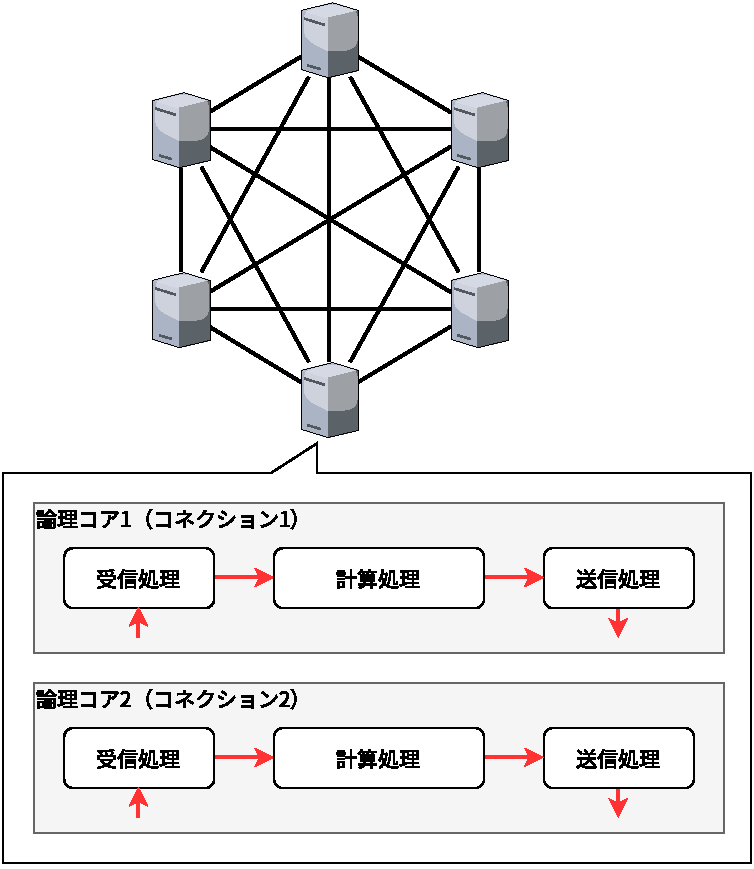
\includegraphics[width=\columnwidth]{pictures/Proposed.pdf}
  \caption{提案手法}
  \label{fig:Proposed}
\end{figure}
